\newpage
\begin{figure}[h]
	\centering
	\caption{UCA 8 - Tracciamento posizione}
	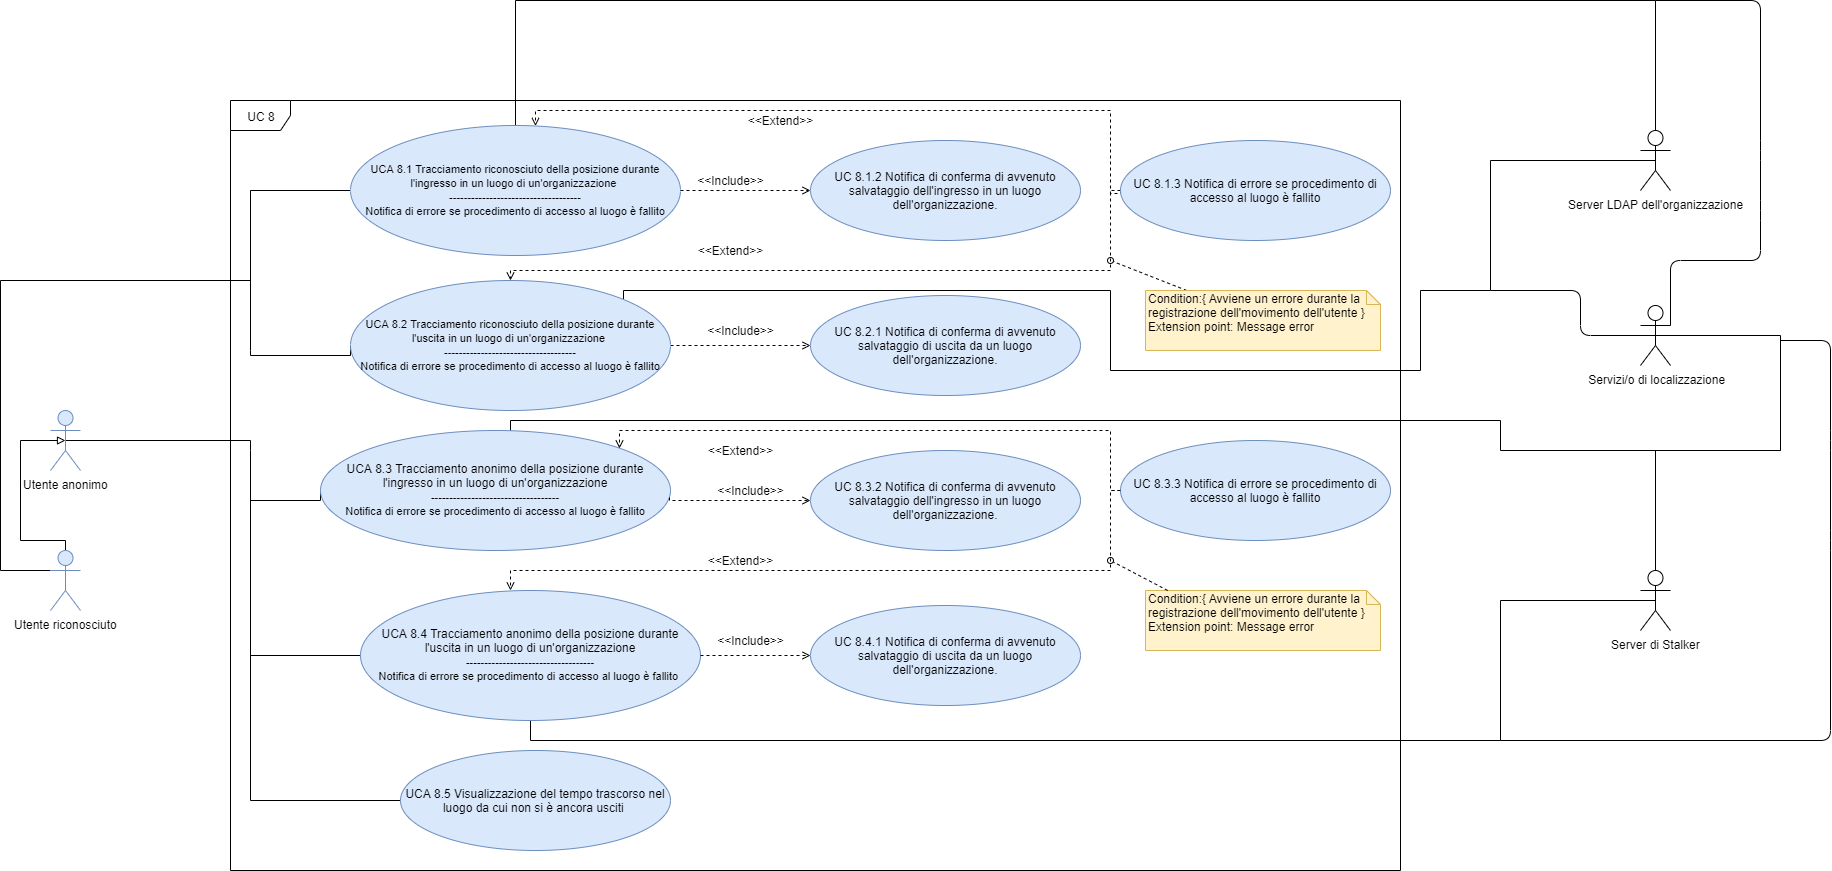
\includegraphics[scale=0.28]{sezioni/UseCase/Immagini/UCA8.png}
\end{figure}
\section{UCA 8 - Tracciamento posizione}%kite level
\begin{itemize}
\item \textbf{Attori primari:} Utente anonimo e Utente riconosciuto;
\item \textbf{Attori secondari:} Servizi/o di localizzazione (GPS, rete cellulare, beacon Bluetooth);
\item \textbf{Precondizione:} L'utente precendetemente autenticato entra in un organizzazione tracciata dall'applicazione, perciò l'utente inizia essere tracciato;
\item \textbf{Postcondizione:} Viene memorizzato dal sistema i timestamp del momento in cui sono avvenuti i tracciamenti, il luogo in cui e’ avvenuto, e il tempo trascorso nel luogo;
\item \textbf{Scenario principale:} L'utente entra in un organizzazione tracciata dall'applicazione, perciò l'utente inizia essere tracciato. Viene salvato il timestamp di entrata e uscita dall'organizzazione e viene salvato il tempo trascorso all'interno dell'organizzazione;
\end{itemize}

\subsection{UCA 8.1 - Tracciamento riconosciuto della posizione durante l'ingresso in un luogo di un'organizzazione}%sea level
\begin{itemize}
\item \textbf{Attori primari:} Utente riconosciuto;
\item \textbf{Attori secondari:} Servizi/o di localizzazione (GPS, rete cellulare, beacon Bluetooth) , Server LDAP dell'organizzazione;
\item \textbf{Precondizione:} L'utente precendetemente autenticato come riconosciuto entra in un organizzazione tracciata dall'applicazione, perciò l'utente inizia essere tracciato;
\item \textbf{Postcondizione:} Viene registrato che l'utente riconosciuto è entrato nel luogo dell'organizzazione in una certa ora e data (timestamp);
\item \textbf{Scenario principale:}
	\begin{itemize}
	\item L'utente riconosciuto con credenziali LDAP entra in un luogo di una organizzazione; tracciata
	\item Viene inviata la data e ora di ingresso e il luogo[UCA 8.1.1];
	\item Viene registrato il timestamp.
\end{itemize}
\item \textbf{Scenario alternativo:} L'invio del timestamp non va a buon fine perchè:
\begin{enumerate}
	\item C'è stato un errore nell'invio del timestamp.
\end{enumerate}
\item \textbf{Estensioni:}
	\begin{enumerate}
		\item UCA 8.1.3 Notifica di errore se procedimento di accesso al luogo è fallito.
	\end{enumerate}
\item \textbf{Inclusioni:}
\begin{enumerate}
	\item UCA 8.1.2 Notifica di conferma di avvenuto salvataggio dell'ingresso in un luogo dell'organizzazione.
\end{enumerate}
\end{itemize}

\subsubsection{UCA 8.1.1 - Invio timestamp LDAP}%fish level
\begin{itemize}
\item \textbf{Attori primari:} Utente riconosciuto;
\item \textbf{Attori secondari:}  Servizi/o di localizzazione (GPS, rete cellulare, beacon Bluetooth), Server LDAP dell'organizzazione;
\item \textbf{Precondizione:} L'utente precendetemente autenticato come riconosciuto, viene inviato un timestamp per registare un suo movimento;
\item \textbf{Postcondizione:} Viene registrato un movimento dell'utente riconosciuto nell'organizzazione in una certa ora e data (timestamp).
\end{itemize}

\subsubsection{UCA 8.1.2 - Notifica di conferma di avvenuto salvataggio dell'ingresso in un luogo dell'organizzazione}%fish level
\begin{itemize}
	\item \textbf{Attori primari:} Utente riconosciuto;
	\item \textbf{Attori secondari:} Server LDAP dell'organizzazione;
	\item \textbf{Precondizione:} L'utente riconosciuto entra in un organizzazione tracciata dall'applicazione, e viene  inviato correttamente il timestamp;
	\item \textbf{Postcondizione:} L'utente viene informato che è stato registrato il suo accesso nell'organizzazione.
\end{itemize}

\subsubsection{UCA 8.1.3 - Notifica di errore se procedimento di accesso al luogo è fallito}%fish level
\begin{itemize}
	\item \textbf{Attori primari:} Utente riconosciuto;
	\item \textbf{Attori secondari:} Servizi/o di localizzazione (GPS, rete cellulare, beacon Bluetooth) , Server LDAP dell'organizzazione;
	\item \textbf{Precondizione:} Avviene un errore durante la registrazione dell'movimento dell'utente
	\item \textbf{Postcondizione:} Viene notificato l'errore all'utente
\end{itemize}

\subsection{UCA 8.2 - Tracciamento riconosciuto della posizione durante l'uscita in un luogo di un'organizzazione}%sea level
\begin{itemize}
	\item \textbf{Attori primari:} Utente riconosciuto;
	\item \textbf{Attori secondari:} Servizi/o di localizzazione (GPS, rete cellulare, beacon Bluetooth), Server LDAP dell'organizzazione;
	\item \textbf{Precondizione:} L'utente precendetemente autenticato come riconosciuto esce da un'organizzazione tracciata dall'applicazione, perciò l'utente smette di essere tracciato;
	\item \textbf{Postcondizione:} Viene registrato che l'utente riconosciuto è uscito dal luogo dell'organizzazione in una certa ora e data (timestamp)
	\item \textbf{Scenario principale:}
	\begin{itemize}
		\item L'utente riconosciuto con credenziali LDAP esce da un luogo di una organizzazione; tracciata
		\item Viene inviata la data e ora di uscita e il luogo[UCA 8.1.1];
		\item Viene registrato il timestamp.
	\end{itemize}
	\item \textbf{Scenario alternativo:} L'invio del timestamp non va a buon fine perchè:
	\begin{enumerate}
		\item C'è stato un errore nell'invio del timestamp.
	\end{enumerate}
	\item \textbf{Estensioni:}
	\begin{enumerate}
		\item UCA 8.1.3 Notifica di errore se procedimento di accesso al luogo è fallito.
	\end{enumerate}
	\item \textbf{Inclusioni:}
	\begin{enumerate}
		\item UCA 8.2.1 Notifica di conferma di avvenuto salvataggio dell'uscita da un luogo dell'organizzazione.
	\end{enumerate}
\end{itemize}

\subsubsection{UC 8.2.1 - Notifica di conferma di avvenuto salvataggio dell'uscita da un luogo dell'organizzazione}%fish level
\begin{itemize}
	\item \textbf{Attori primari:} Utente riconosciuto;
	\item \textbf{Attori secondari:} Server LDAP dell'organizzazione;
	\item \textbf{Precondizione:} L'utente riconosciuto esce da un'organizzazione tracciata dall'applicazione, e viene  inviato correttamente il timestamp;
	\item \textbf{Postcondizione:} L'utente viene informato che è stato registrato che è uscito dall'organizzazione.
\end{itemize}

\subsection{UCA 8.3 - Tracciamento anonimo della posizione durante l'ingresso in un luogo di un'organizzazione}%sea level
\begin{itemize}
	\item \textbf{Attori primari:} Utente anonimo; 
	\item \textbf{Attori secondari:} Servizi/o di localizzazione (GPS, rete cellulare, beacon Bluetooth);
	\item \textbf{Precondizione:} L'utente precendetemente autenticato come anonimo entra in un organizzazione tracciata dall'applicazione, perciò l'utente inizia essere tracciato;
	\item \textbf{Postcondizione:} Viene registrato che l'utente anonimo è entrato nel luogo dell'organizzazione in certa ora e data (timestamp)
	\item \textbf{Scenario principale:}
	\begin{itemize}
		\item L'utente anonimo entra in un luogo di una organizzazione tracciata;
		\item Viene inviata la data e ora di ingresso e il luogo[UCA 8.3.1];
		\item Viene registrato il timestamp.
	\end{itemize}
	\item \textbf{Scenario alternativo:} L'invio del timestamp non va a buon fine perchè:
	\begin{enumerate}
		\item C'è stato un errore nell'invio del timestamp.
	\end{enumerate}
	\item \textbf{Estensioni:}
	\begin{enumerate}
		\item UCA 8.3.3 Notifica di errore se procedimento di accesso al luogo è fallito.
	\end{enumerate}
	\item \textbf{Inclusioni:}
	\begin{enumerate}
		\item UCA 8.3.2 Notifica di conferma di avvenuto salvataggio dell'ingresso in un luogo dell'organizzazione.
	\end{enumerate}
\end{itemize}

\subsubsection{UCA 8.3.1 - Invio timestamp LDAP}%fish level
\begin{itemize}
	\item \textbf{Attori primari:} Utente anonimo;
	\item \textbf{Attori secondari:}  Servizi/o di localizzazione (GPS, rete cellulare, beacon Bluetooth), Server di Stalker;
	\item \textbf{Precondizione:} L'utente precendetemente autenticato come anonimo, viene inviato un timestamp per registare un suo movimento;
	\item \textbf{Postcondizione:} Viene registrato un movimento dell'utente anonimo nell'organizzazione in una certa ora e data (timestamp).
\end{itemize}

\subsubsection{UCA 8.3.2 - Notifica di conferma di avvenuto salvataggio dell'ingresso in un luogo dell'organizzazione}%fish level
\begin{itemize}
	\item \textbf{Attori primari:} Utente anonimo;
	\item \textbf{Attori secondari:} Server di Stalker;;
	\item \textbf{Precondizione:} L'utente anonimo entra in un organizzazione tracciata dall'applicazione, e viene  inviato correttamente il timestamp;
	\item \textbf{Postcondizione:} L'utente viene informato che è stato registrato il suo accesso nell'organizzazione.
\end{itemize}

\subsubsection{UCA 8.3.3 - Notifica di errore se procedimento di accesso al luogo è fallito}%fish level
\begin{itemize}
	\item \textbf{Attori primari:} Utente anonimo;
	\item \textbf{Attori secondari:} Servizi/o di localizzazione (GPS, rete cellulare, beacon Bluetooth) , Server di Stalker;;
	\item \textbf{Precondizione:} Avviene un errore durante la registrazione dell'movimento dell'utente
	\item \textbf{Postcondizione:} Viene notificato l'errore all'utente
\end{itemize}

\subsection{UCA 8.4 - Tracciamento anonimo della posizione durante l'uscita in un luogo di un'organizzazione} %sea level
\begin{itemize}
	\item \textbf{Attori primari:} Utente anonimo 
	\item \textbf{Attori secondari:} Servizi/o di localizzazione (GPS, rete cellulare, beacon Bluetooth), Server di Stalker;
	\item \textbf{Precondizione:} L'utente precendetemente autenticato come anonimo esce da un'organizzazione tracciata dall'applicazione, perciò l'utente smette di essere tracciato;
\item \textbf{Postcondizione:} Viene registrato che l'utente anonimo è uscito dal luogo dell'organizzazione in una certa ora e data (timestamp)
\item \textbf{Scenario principale:}
\begin{itemize}
	\item L'utente anonimo entra in un luogo di una organizzazione tracciata;
	\item Viene inviata la data e ora di uscita e il luogo[UCA 8.3.1];
	\item Viene registrato il timestamp.
\end{itemize}
\item \textbf{Scenario alternativo:} L'invio del timestamp non va a buon fine perchè:
\begin{enumerate}
	\item C'è stato un errore nell'invio del timestamp.
\end{enumerate}
\item \textbf{Estensioni:}
\begin{enumerate}
	\item UCA 8.3.3 Notifica di errore se procedimento di accesso al luogo è fallito.
\end{enumerate}
\item \textbf{Inclusioni:}
\begin{enumerate}
	\item UCA 8.4.1 Notifica di conferma di avvenuto salvataggio dell'uscita da un luogo dell'organizzazione.
\end{enumerate}
\end{itemize}

\subsubsection{UC 8.4.1 - Notifica di conferma di avvenuto salvataggio dell'uscita da un luogo dell'organizzazione}%fish level
\begin{itemize}
\item \textbf{Attori primari:} Utente anonimo;
\item \textbf{Attori secondari:} Server di Stalker;
\item \textbf{Precondizione:} L'utente anonimo esce da un'organizzazione tracciata dall'applicazione, e viene  inviato correttamente il timestamp;
\item \textbf{Postcondizione:} L'utente viene informato che è stato registrato che è uscito dall'organizzazione.
\end{itemize}

\subsection{UCA 8.5 - Visualizzazione del tempo trascorso nel luogo da cui non si è ancora usciti}%sea level
\begin{itemize}
	\item \textbf{Attori primari:} Utente anonimo e Utente riconosciuto;
	\item \textbf{Precondizione:} L'utente autenticato si trova all'interno di una organizzazione tracciata dall'applicazione e vuole sapere quanto tempo ha trascorso nel luogo in cui si trova;
	\item \textbf{Postcondizione:} Viene riportato all'utente quanto tempo ha trascorso nel luogo in cui si trova;
	\item \textbf{Scenario principale:}
	\begin{itemize}
		\item L'utente accede alla funzionalità di "Visualizzazione del tempo trascorso nel luogo";
		\item Viene mostrato il tempo che ha trascorso nel luogo.
	\end{itemize}
\end{itemize}

